\chapter{Implementering}
\section{Hardware}
\label{HW_Implementering}
På figur \ref{fig:Pololu-A4988} ses hvordan Pololu-A4988 opsættes til PSoC 5LP og en motor. I den endelige impementering er antallet af Pololu-A4988 motor drivere og motorer i forholdet 1:1. Driveren fungerer som bindeled mellem PSoC 5LP og motoren. Tabel \ref{tab:Pololu-A4988_pin_configuration} viser pin konfigureringen fra Pololu-A4988 til henholdsvis PSoC 5LP og 28BYJ-48. Rækkefølgen af pins i tabellen svarer til billedet fra figur \ref{fig:Pololu-A4988} læst fra øverste venstre hjørne. MS1, MS2 og MS3 er ikke forbundet til noget. RESET og SLEEP er forbundet til hinanden.

\begin{figure}[H]
	\centerline{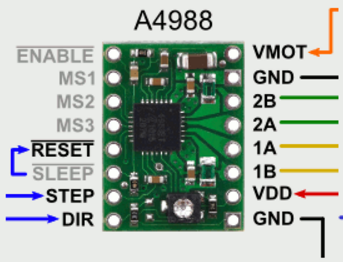
\includegraphics[scale=0.6]{Pololu-A4988.png}}
	\caption[]{Pololu-A4988}\footnotemark
	\label{fig:Pololu-A4988}
\end{figure}
\footnotetext{https://forum.pololu.com/t/a4988-issue/6518}

\begin{table}[H]
  \centering
\begin{tabular}{ |l|c|c|c| }
  \hline
   & \textbf{PSoC 5LP} & \textbf{Motor} & \textbf{VDD} \\
  \hline 
  ENABLE & X & & \\
  \hline
  STEP & X & & \\
  \hline
  DIR & X & & \\
  \hline
  VMOT (10V) & & & X \\
  \hline
  GND & X & & X \\
  \hline
  2B & & X & \\
  \hline
  2A & & X & \\
  \hline
  1A & & X & \\
  \hline
  1B & & X & \\
  \hline
  VDD (5V) & & & X \\
  \hline
  GND & & & X \\
  \hline
\end{tabular}
\caption{Pololu-A4988 pin konfigurering}\label{tab:Pololu-A4988_pin_configuration}
\end{table}

\noindent
VDD er altså spændingsforsyning som leverer både 5V og 10V til henholdsvis driveren og motoren.
\\
\\
Sensorerne har tre pins som alle er sat direkte til PSoC 5LP Master, som vist i tabel \ref{tab:Sensor_pin_konfigurering}.

\begin{table}[H]
  \centering
\begin{tabular}{ |l|c| }
  \hline
  \textbf{GP2Y0A21YK Sensor} & \textbf{PSoC 5LP}\\
  \hline 
  $V_0$ & P[X:X] \\
  \hline 
  GND & P[X:X] \\
  \hline 
  $V_CC$ & P[X:X] \\
  \hline 
\end{tabular}
\caption{GP2Y0A21YK sensor implementeret med PSoC 5LP}\label{tab:Sensor_pin_konfigurering}
\end{table}